\chapter{Existing Embedded Technologies}
There already exists embedded microcontrollers capable of running Linux. Big companies as for example ARM, Qualcomm, MediaTek, Intel and AMD have created microcontroller capable of running Linux. But the processor architecture of those microcontrollers is not open-source, much less the microcontroller itself. 

As an example, the \textit{Raspberry Pi 4} is a very capable and cheap board where a developer can test and implement new software running in Linux. The Raspberry \acrshort{cpu} is an \textit{Cortex-A72}~\cite{cortex_a72} witch is a System on Chip (SoC) developed by ARM on their ARMv8 64-bit CPU architecture. But if someone wanted to use the Raspberry as a base for his costume hardware design, that would be impossible. And thus appears the need for open-source hardware that allows creating something new without having to start from scratch every time. This led to the appearance of RISC-V the open-source CPU architecture.


\section{Closed source RISC-V Embedded Systems}
Since then, a few companies using RISC-V have appeared. RISC-V CPUs are already present in the automotive and IoT markets, besides AI chips in data centers. Due to the RISC-V ISA royalty free license new StartUps tend to look at RISC-V CPUs as a solution for their cores. Even if the CPU Core isn't free to use it ends up being a cheaper solution.

While creating new products companies proved how advantageous the RISC-V architecture was. Furthermore, they have contributed to open-source software, hardware and documentation. Some companies with a big recognitions involved with RISC-V technology are:
\begin{itemize}
    \item \textit{Western Digital} who now uses RISC-V in its external storage disks. 
    \item \textit{Microchip} as launched the first RISC-V-Based System-on-Chip (SoC) FPGA, \textit{PolarFire}. 
    \item \textit{Antmicro/Microsemi}~\footnote{Microchip has acquired Microsemi Corporation in May 2018.} have built a software called Renode that is used to develop, debug and test multi-node RISC-V device systems.
    \item \textit{BeagleBoard.org}, \textit{Seeed Studio} and \textit{StarFive} worked together to build the first affordable RISC-V computer designed to run Linux, \textit{BeagleV}~\cite{beagleV}. The board is priced around 150€.
\end{itemize}

These companies have all helped pave the way for a full-feature Operating System based on the Linux kernel to be compatible with the RISC-V architecture. However, there are two companies that have a bigger impact on RISC-V CPU design, those are Andes Technology and SiFive.

\subsection{Andes Technology}
Andes Technology is one of the founder members of the RISC-V International. Since it is highly involved with RISC-V it ended up being one of the major contributor (and maintainer) of the RISC-V tool-chain. This is important because the RISC-V ISA is merely an instruction set architecture, there needs to exist complementing software, such as compiler and development tools.

Nowadays Andes CPU's are applied nearly everywhere, from telecommunications, storage controllers, touch screen sensors to data centers, etc. Andes Technologies has had incredible success using RISC-V technology, as prove they have shipped billions of embedded SoC with RISC-V processors based on their RISC-V ISA variant, AndeStar™ V5. 

Andes CPUs witch are capable of running Linux are the \textit{A25}~\cite{a25} and \textit{AX25}~\cite{ax25}. Both support single and double precision floating point, the RISC-V P-extension (draft) DSP/SIMD ISA and an MMU (Memory Management Unit) for Linux applications. Besides that both enable the use of Machine (M), User (U) and Supervisor (S) Privilege levels that allow running Linux and other advanced operating systems with protection between kernel and user programs. Furthermore, both have L1 instruction and data cache. The difference between them is that \textit{A25} is based on 32-bit architecture and the \textit{AX25} is 64-bit. This leads to the \textit{AX25} being ideal for embedded applications that need to access address space over 4GB, and the \textit{A25} being smaller in gate count. Both CPUs can be implemented on the AE350~\cite{ae350} SoC allowing to use these CPUs on developer boards, for example in the \textit{ADP-XC7K160/410}~\cite{adp-xc7k160}.

\subsection{SiFive}
SiFive is a company that was born from the RISC-V ISA. SiFive was founded by three researchers from the University of California Berkeley, Krste Asanović, Yunsup Lee, and Andrew Waterman. Those researchers were deeply involved with the development of the RISC-V ISA, from working on the base ISA to working on the floating point numbers and compressed instructions ISA extensions. It is no surprise that the first company to release a chip and development board that implemented the RISC-V ISA was SiFive. This happened in 2016 one year after the company was founded.

In 2017 SiFive launched \textit{U54}~\cite{u54} witch was the first RISC-V CPU capable of running a full fledge Operating System like Linux. With it they launched the \textit{U54-MC}~\cite{u54-mc} SoC that had four \textit{U54} 64-bit cores. Furthermore, the \textit{U54-MC} implemented the initial CLINT and PLIC unit. The development of the \acrshort{clint} and the \acrshort{plic} made by SiFive would eventually lead to the documentation and specification of the respective hardware components with witch RISC-V systems must be compliant if they proclaim to use either one. One year after, in 2018, they launched \textit{HiFive Unleashed}~\cite{hifive_unleashed} witch was the first board that implemented the \textit{U54} CPU and run a Linux OS with a desktop environment (DE). The \textit{HiFive Unleashed} has been discontinued and better hardware has been made available.

SiFive has since then extended their \textit{U Cores} product lineup. All \textit{U} cores are 64-bit application processors capable of running Linux. The highest performance core is the \textit{U74}~\cite{u74}. The core architecture is RV64GBC witch means it supports the RISC-V I, M, A, F, D, B and C ISA extensions (explained in \textbf{*ref section 2.3.x*}). This CPU has already been applied to multiple boards, for example, the \textit{BeagleV} has a \acrshort{soc} with dual core SiFive \textit{U74} CPU. SiFive as also launched its own development board, \textit{HiFive Unmatched}~\cite{hifive_unmatched}, with four \textit{U74} cores on the \textit{U74-MC}~\cite{u74-mc} SoC. Furthermore, in 2021, Canonical the developers behind Ubuntu have announced the OS support for both the HiFive Unmatched and HiFive Unleashed.

\section{Open-Source Solutions}
Built upon the RISC-V open-source \acrlong{isa}, various CPU designs have emerged. Some of them are fully open-source and might be implemented in other projects. Those CPUs were mostly developed by Universities research groups or by individuals with a grant. 

RISC-V CPUs are most popular in embedded systems and IoT devices. Consequently there exists a widely variety of open-source CPUs witch are implemented on multiple embedded microcontrollers. A few examples of those \acrshort{cpu}s would be the \textit{PicoRV32}~\cite{picorv32}, \textit{NEORV32}~\cite{neorv32}, \textit{DarkRISCV}~\cite{darkriscv} and \textit{Ibex}~\cite{ibex} from lowRISC. But those will not be discussed in detail on this paper since they do not meet the requirements to run the Linux Kernel. This \acrshort{cpu}s either only support \acrfull{machine} level privilege mode or support \acrfull{machine}+\acrfull{supervisor} mode. Moreover, none of the given examples support the Atomic RISC-V \acrshort{isa} extension. This extension is essential to run Linux. Since the kernel explicitly executes instructions from the Atomic extension. 

To run a Linux based Operating System an application processor is needed. A \acrshort{cpu} is considered an application processor if it has the hardware required to run a full-feature \acrfull{os} and user applications. This means that the processor should have the required \acrfull{csr}, support \acrshort{machine}+\acrshort{supervisor}+\acrshort{user} privilege modes and support atomic instructions. An open-source solution would be either the \textit{CVA6}~\cite{zaruba2019cost} (previously known as Ariane), \textit{BOOM}~\cite{zhaosonicboom} or \textit{VexRiscv}~\cite{vexriscv}.

\subsection{\textit{CVA6}}
The CVA6 is a 6-stage, single issue, in-order CPU which can execute either the 32-bit or 64-bit RISC-V instruction set. CVA6 has support for the I, M, A and C RISC-V \acrshort{isa} extensions. The original design was initiated in a research group by a Phd student at ETH Zurich (where they called the core Ariane). Since then the development and maintenance of CVA6 was incorporated in the \textit{OpenHW Group} as part of their CORE-V processor lineup. The support for RV32IMAC was only developed recently by Thales, and is also open-source. The \acrshort{cpu} design is illustrated in figure \ref{fig:cva6_design} that was obtained from: \url{https://github.com/openhwgroup/cva6/}.

\begin{figure}[!h]
    \centering
    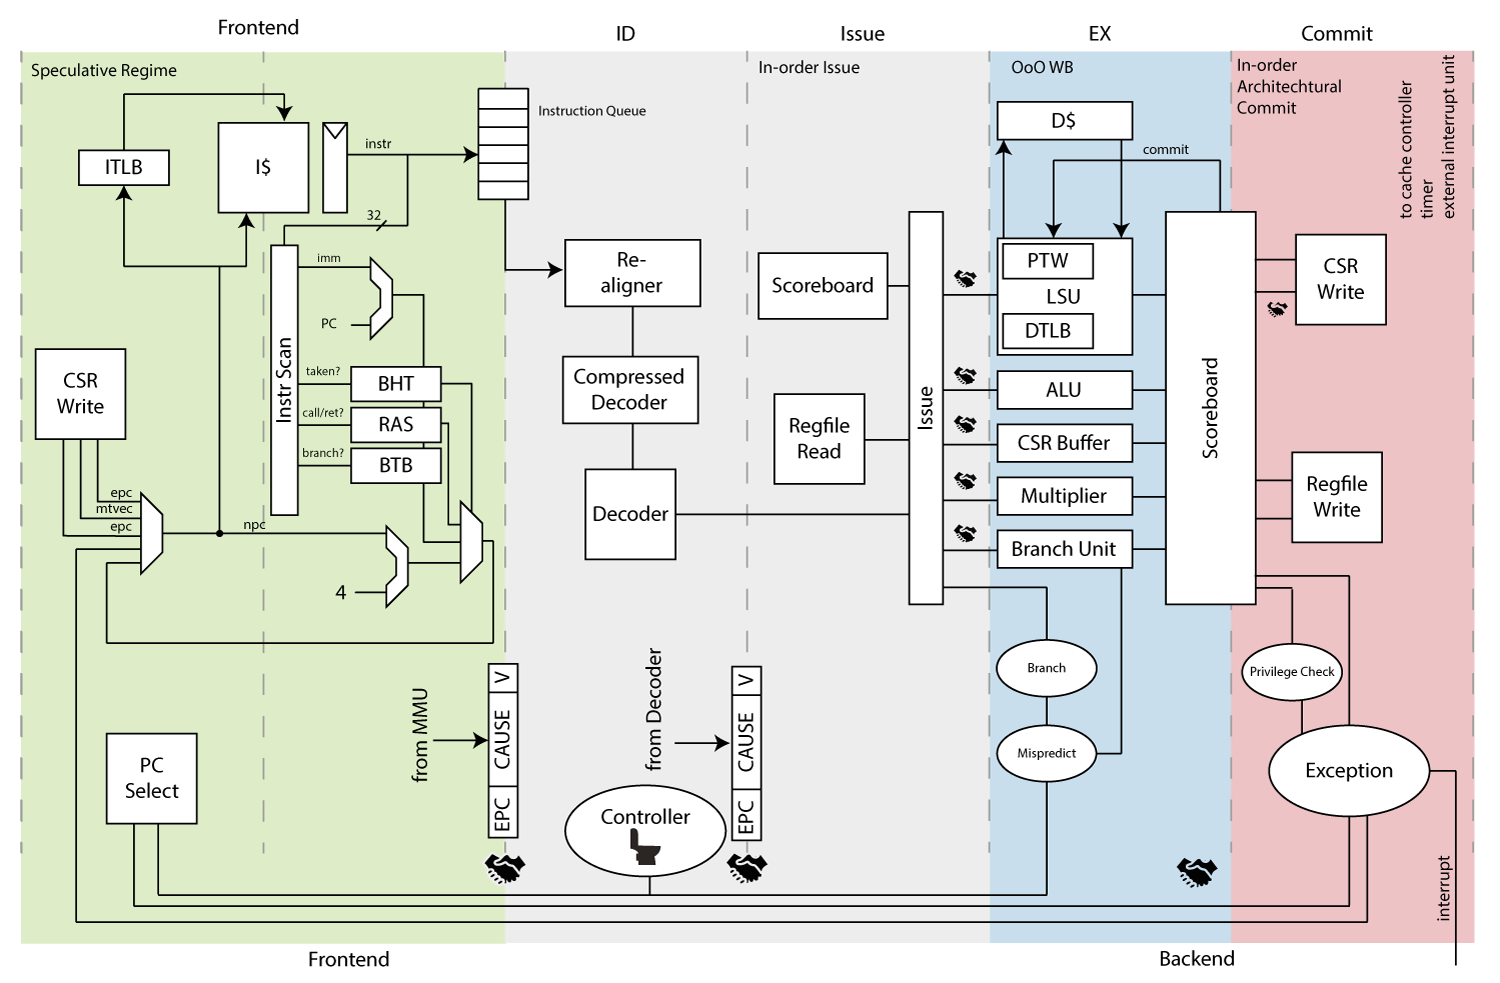
\includegraphics[width=0.7\linewidth]{cva6_design.png}
    \caption{CVA6 core design architecture}
    \label{fig:cva6_design}
\end{figure}

The CVA6 supports any operating system based on Unix since it implements the three needed privilege levels M, S and U. The core is written in SystemVerilog, and its micro-architecture is designed to reduce the critical path length. Since it is written in SystemVerilog, it is easier for someone knowledgeable in the classic Verilog and VHDL languages to understand and create a customized CPU based on the CVA6, than if it was written in a high level hardware description language. However, although the CVA6 is an open-source project it is hard to take advantage of isolated hardware components. This is as  a consequence of how it was developed. Every SystemVerilog module of the CVA6 depends on other files from the project and the CPU itself is very little customizable. To illustrate the problem if we wanted to remove the L1 cache present in the CVA6 in order to use the L1 cache used on IOb-SoC, it would be very difficult and time consuming to create a CPU core without that component.

The CVA6 can be found implemented on \textit{OpenPiton}~\cite{Balkind:2016:OOS:2872362.2872414}. \textit{OpenPiton} is an open-source project developed by the Princeton Parallel Group. With it one can easily create a SoC that has multiple CV6 cores and run a full-feature \acrfull{os} on a development board with an FPGA.

\subsection{The Berkeley Out-of-Order RISC-V Processor}
The Berkeley Out-of-Order RISC-V Processor (\textit{BOOM}~\cite{zhaosonicboom}) is a superscalar \acrfull{ooo} processor executing the RV64GC variant of the RISC-V ISA. BOOM was created at the University of California, Berkeley in the Berkeley Architecture Research group. The CPU design is optimized to run on ASICs, although it can also be implemented on FPGAs. Its priority is to be a high performance, synthesizable, and parametrizable core for architecture research. The current release, named \textit{SonicBOOM}, has one of the best performance from the publicly available open-source RISC-V cores.

BOOM is a 10-stage CPU with the following stages: Fetch, Decode, Register Rename, Dispatch, Issue, Register Read, Execute, Memory, Writeback, and Commit. However, in most practical implementations, many of those stages are merged, generating seven stages altogether: Fetch, Decode/Rename, Rename/Dispatch, Issue/Register Read, Execute, Memory and Writeback. Since committing happens asynchronously, it is not counted as part of the \enquote{pipeline}. The load-store unit is optimized for the superscalar out-of-order architecture, and the data cache is organized into two dual-ported banks. At the front end, it is possible to customize the size of the L1 Instruction cache, the TLB, and the decode stage. Similarly to the CVA6, it is difficult or impossible to remove the cache from the core design and use the IOb-Cache instead. 

This \acrshort{cpu} design is written in Chisel~\cite{bachrach2012chisel} \acrfull{hdl}. The \acrfull{chisel} allows to produce synthesizable Verilog designs while using a high level language to describe the hardware. \acrshort{chisel} is an adaptation of Scala~\cite{odersky2004scala} programing language, adding hardware construction primitives. 

To build a \acrfull{soc} with BOOM we would have to utilize the \textit{Rocket Chip}~\cite{asanovic2016rocket} SoC generator from CHIPS Alliance. Since BOOM uses micro-architecture structures (TLBs, PTWs, etc) from that tool.

\subsection{\textit{VexRiscv}}
The \textit{VexRiscv}~\cite{vexriscv} CPU is a 32-bit Linux Capable RISC-V CPU written in the \textit{SpinalHDL}~\cite{papon2017spinalhdl}. The hardware description of this CPU is accomplished by utilizing a software-oriented approach. Similarly to \acrshort{chisel}, \textit{SpinalHDL} is based on the Scala programing language. 

VexRiscv is an in-order CPU with five \enquote{pipeline} stages. Many CPU plugins are optional, which add many functionalities to build a custom RISC-V CPU. The architecture design approach in this processor is unconventional, but it has its benefits: there are remarkably few fixed hardware components; Parts of the CPU can be swapped, turned on and turned off via the plugin system; without modifying any of the CPU sources, it is possible to add new functionalities/instructions easily; It permits the CPU arrangement to cover a significantly large spectrum of implementations, allowing the construction of an entirely parametrized CPU design. When the CPU is configured without plugins, it only includes the description of the five \enquote{pipeline} stages and their basic functionalities and nothing else. Everything else needs to be added to the CPU via plugins, including the program counter. VexRiscv can either be an application processor capable of running a full-feature \acrfull{os} or a super simple microprocessor ideal for bare-bone applications depending on the way it is configured. Contrary to \textit{BOOM}, \textit{VexRiscv} does not need any external library. This makes it very easy to generate the synthesizable Verilog file from a \textit{SpinalHDL} design.

There exists an open-source project that runs Linux with \textit{VexRiscv}, \textit{linux-on-litex-vexriscv}~\cite{litex_vexriscv}. \textit{LiteX} is used to create a \acrfull{soc} around the \textit{VexRiscv} core. \textit{LiteX} \acrshort{soc} design and peripherals are written in \textit{Migen}~\cite{bourdeauducq2012migen} another hight level \acrshort{hdl}. \textit{Migen} unlike \textit{SpinalHDL} and  \acrshort{chisel} is based on Python 3.5. On account of the language describing its hardware and the way the \textit{linux-on-litex-vexriscv} project is structured it is very hard to understand how the system works, where the generated \acrshort{rtl} is and how to add custom hardware. Furthermore, \textit{linux-on-litex-vexriscv} uses \acrshort{fpga} specific hardware, making it impossible to port the system to \acrshort{asic}.

Recently the developer behind \textit{SpinalHDL} has also made public the \textit{NaxRiscv} \acrshort{cpu}. \textit{NaxRiscv} is a \acrshort{cpu} designed specifically to run a full-feature \acrlong{os}, like Linux. And just like \textit{VexRiscv}, \textit{NaxRiscv} uses \textit{SpinalHDL} to describe its hardware. Although \textit{NaxRiscv} seems like a very promising \acrshort{cpu} it is still on its early stages. Consequently it has a primitive interface witch makes it complicated to implement on costume \acrfull{soc}.


\section{Overall CPU comparison}
In table \ref*{tab:cpu_comparison} we can see a comparison of the \acrshort{cpu}s that were presented in the previous sections, capable of running a full-feature \acrfull{os}. All of the CPUs on the table are considered an application processor. It can be observed that every CPU has a \acrfull{mmu} and they all support \acrshort{user}+\acrshort{supervisor}+\acrshort{machine} privilege mode. Furthermore, all of the \acrshort{cpu}s hardware design have L1 Instruction Cache and L1 Data cache system integrated. This happens because to support atomic instructions it is easier to have direct access to the L1 Cache.

\textit{GNU/Linux} is the combinations of \textit{GNU} with the Linux kernel. The GNU Project developed a large parte of the software that forms a complete \acrfull{os}. Many \enquote{Linux} distributions make use of that software, a few examples would be \textit{Debian}, \textit{Ubuntu}, \textit{openSUSE}, \textit{Fedora}, and the list could go on. So a processor that supports the GNU/Linux feature is a CPU that is capable of running a distribution like \textit{Ubuntu} or \textit{Debian}. From the table we can see that 32-bit RISC-V \acrshort{cpu}s are the only ones not capable of running a \textit{GNU/Linux} \acrfull{os}.

\begin{table}[!ht]
    \centering
    \resizebox{\textwidth}{!}{%
    \begin{tabular}{cccccccccc}
        & ARM                             & \multicolumn{2}{c}{Andes Technology}                      & \multicolumn{2}{c}{SiFive}                                & PULP platform                 & UC Berkeley                 & \multicolumn{2}{c}{SpinalHDL}                                 \\ \cline{2-10} 
\multicolumn{1}{c|}{}                                                                   & \multicolumn{1}{c|}{Cortex-A72} & \multicolumn{1}{c|}{A25}    & \multicolumn{1}{c|}{AX25}   & \multicolumn{1}{c|}{U54}    & \multicolumn{1}{c|}{U74}    & \multicolumn{1}{c|}{CVA6}      & \multicolumn{1}{c|}{BOOM}   & \multicolumn{1}{c|}{VexRiscv} & \multicolumn{1}{c|}{NaxRiscv} \\ \hline
\multicolumn{1}{|c|}{\begin{tabular}[c]{@{}c@{}}Architecture\\ bit widths\end{tabular}} & \multicolumn{1}{c|}{64-bit}     & \multicolumn{1}{c|}{32-bit} & \multicolumn{1}{c|}{64-bit} & \multicolumn{1}{c|}{64-bit} & \multicolumn{1}{c|}{64-bit} & \multicolumn{1}{c|}{32/64-bit} & \multicolumn{1}{c|}{64-bit} & \multicolumn{1}{c|}{32-bit}   & \multicolumn{1}{c|}{64-bit}   \\ \hline
\multicolumn{1}{|c|}{MMU}                                                               & \multicolumn{1}{c|}{Y}          & \multicolumn{1}{c|}{Y}      & \multicolumn{1}{c|}{Y}      & \multicolumn{1}{c|}{Y}      & \multicolumn{1}{c|}{Y}      & \multicolumn{1}{c|}{Y}         & \multicolumn{1}{c|}{Y}      & \multicolumn{1}{c|}{Y}        & \multicolumn{1}{c|}{Y}        \\ \hline
\multicolumn{1}{|c|}{FPU}                                                               & \multicolumn{1}{c|}{Y}          & \multicolumn{1}{c|}{Y}      & \multicolumn{1}{c|}{Y}      & \multicolumn{1}{c|}{Y}      & \multicolumn{1}{c|}{Y}      & \multicolumn{1}{c|}{X}         & \multicolumn{1}{c|}{Y}      & \multicolumn{1}{c|}{X}        & \multicolumn{1}{c|}{Y}        \\ \hline
\multicolumn{1}{|c|}{\begin{tabular}[c]{@{}c@{}}16-bit \\ instructions\end{tabular}}    & \multicolumn{1}{c|}{X}          & \multicolumn{1}{c|}{Y}      & \multicolumn{1}{c|}{Y}      & \multicolumn{1}{c|}{Y}      & \multicolumn{1}{c|}{Y}      & \multicolumn{1}{c|}{Y}         & \multicolumn{1}{c|}{Y}      & \multicolumn{1}{c|}{Y}        & \multicolumn{1}{c|}{X}        \\ \hline
\multicolumn{1}{|c|}{Cache L1(I+D)}                                                     & \multicolumn{1}{c|}{Y}          & \multicolumn{1}{c|}{Y}      & \multicolumn{1}{c|}{Y}      & \multicolumn{1}{c|}{Y}      & \multicolumn{1}{c|}{Y}      & \multicolumn{1}{c|}{Y}         & \multicolumn{1}{c|}{Y}      & \multicolumn{1}{c|}{Y}        & \multicolumn{1}{c|}{Y}        \\ \hline
\multicolumn{1}{|c|}{\begin{tabular}[c]{@{}c@{}}Interrupt \\ Controller\end{tabular}}   & \multicolumn{1}{c|}{X}          & \multicolumn{1}{c|}{Y}      & \multicolumn{1}{c|}{Y}      & \multicolumn{1}{c|}{Y}      & \multicolumn{1}{c|}{Y}      & \multicolumn{1}{c|}{X}         & \multicolumn{1}{c|}{X}      & \multicolumn{1}{c|}{X}        & \multicolumn{1}{c|}{X}        \\ \hline
\multicolumn{1}{|c|}{\acrshort{user}+\acrshort{supervisor}+\acrshort{machine} Mode}                                                        & \multicolumn{1}{c|}{N/A}        & \multicolumn{1}{c|}{Y}      & \multicolumn{1}{c|}{Y}      & \multicolumn{1}{c|}{Y}      & \multicolumn{1}{c|}{Y}      & \multicolumn{1}{c|}{Y}         & \multicolumn{1}{c|}{Y}      & \multicolumn{1}{c|}{Y}        & \multicolumn{1}{c|}{Y}        \\ \hline
\multicolumn{1}{|c|}{GNU/Linux}                                                         & \multicolumn{1}{c|}{Y}          & \multicolumn{1}{c|}{X}      & \multicolumn{1}{c|}{Y}      & \multicolumn{1}{c|}{Y}      & \multicolumn{1}{c|}{Y}      & \multicolumn{1}{c|}{Y}         & \multicolumn{1}{c|}{Y}      & \multicolumn{1}{c|}{X}        & \multicolumn{1}{c|}{Y}        \\ \hline
\multicolumn{1}{|c|}{Open-Source}                                                       & \multicolumn{1}{c|}{X}          & \multicolumn{1}{c|}{X}      & \multicolumn{1}{c|}{X}      & \multicolumn{1}{c|}{X}      & \multicolumn{1}{c|}{X}      & \multicolumn{1}{c|}{Y}         & \multicolumn{1}{c|}{Y}      & \multicolumn{1}{c|}{Y}        & \multicolumn{1}{c|}{Y}        \\ \hline
\end{tabular}%
    }
    \caption{CPU comparison table: Y means the CPU supports the feature; X means the CPU does not supports the feature; N/A means the feature is no applicable to the respective CPU.}
    \label{tab:cpu_comparison}
\end{table}